\documentclass{article}
\usepackage[margin=1.25in]{geometry}
\usepackage{amsmath, amssymb, setspace, enumerate, enumitem}
\usepackage{setspace}
\usepackage{graphicx}
\onehalfspacing

\begin{document}
    \begin{enumerate}
        \item The dimensions of $Z$ are 45
        \item training data:\\
        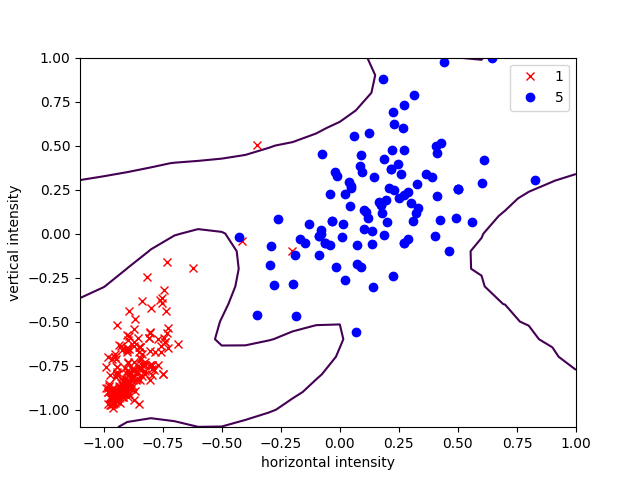
\includegraphics[scale=0.5]{images/reg0train.png}\\
        testing data:\\
        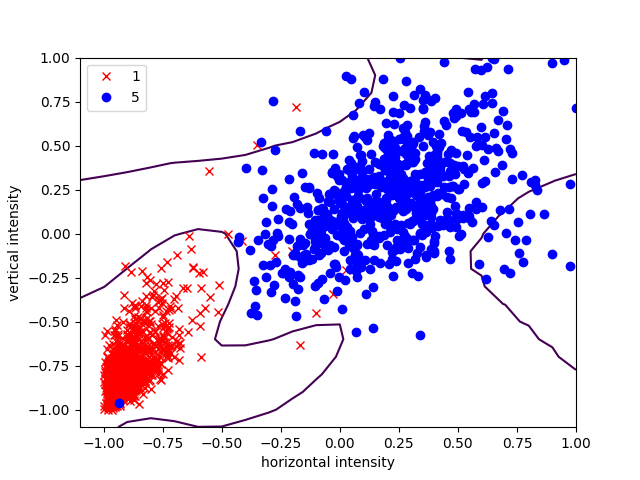
\includegraphics[scale=0.5]{images/reg0test.png}\\
        The data appears to be \textbf{overfitted}
        \item training data:\\
        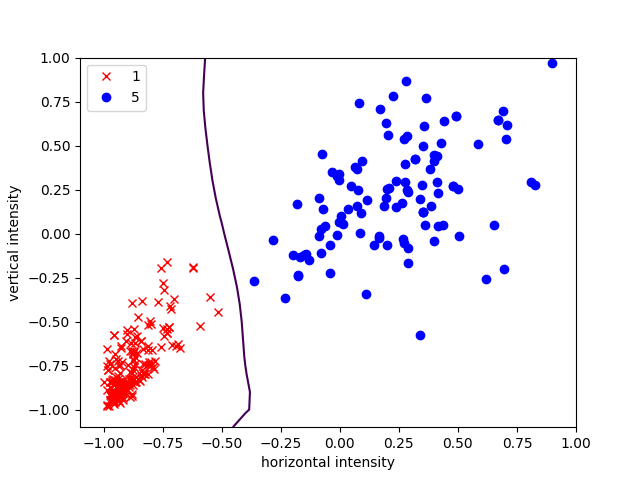
\includegraphics[scale=0.5]{images/reg2train.png}\\
        testing data:\\
        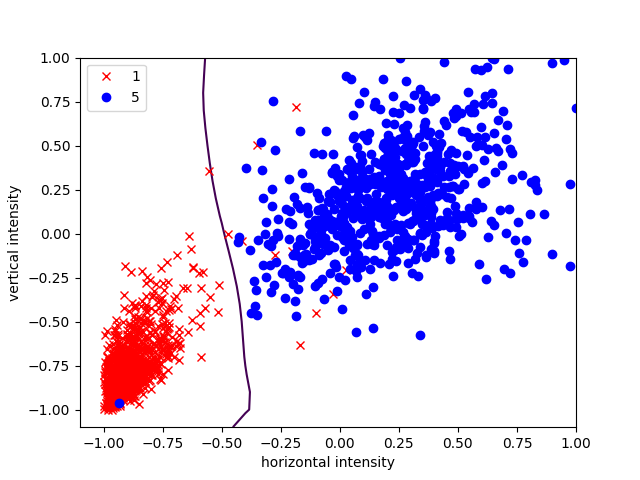
\includegraphics[scale=0.5]{images/reg2test.png}\\
        Data is regularized, there doesn't appear to be any under or overfitting.
        \item Plot:\\ 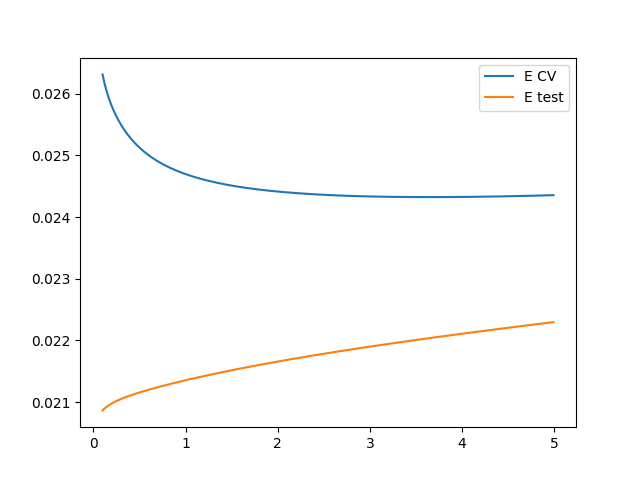
\includegraphics[scale=0.5]{images/CVvsTEST.png}\\
        I chose my values for $\lambda \in \{0, 0.01, 0.02, ..., 5\}$, behavior wise, it appears that as the regularizer increases, the cross validation error decreases, while the regression error onthe test set increases as the regularizer increases.
        \item Plot with $\lambda = 3.64$: \\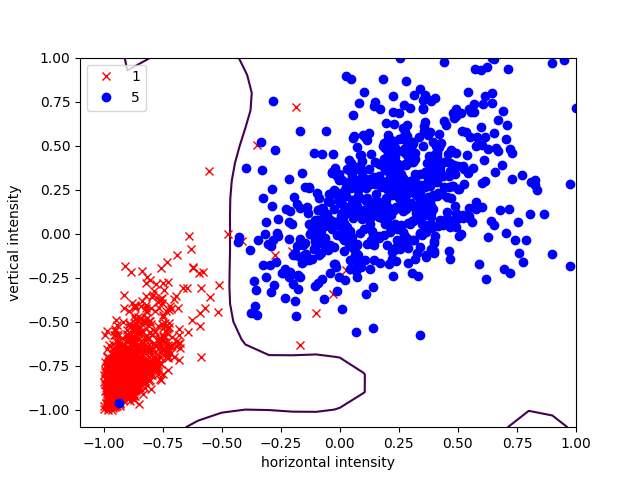
\includegraphics[scale=0.5]{images/bestReg.png}
    \end{enumerate}
\end{document}